\chapter{Quicksort}

\providecommand{\E}{\ensuremath{\mathbb{E}}}

There is a sorting algorithm that, on paper, has a terrible worst case --
quadratic, $\Theta(n^2)$, the same as the clumsy bubble sort you were warned
about. And yet this algorithm is, in practice, the one that ships. It is the
default in countless standard libraries. It sorts arrays faster than almost
anything else with the same asymptotic average. Its name is \emph{quicksort},
and the question of why something with a quadratic worst case earns the word
``quick'' is one of the better stories in algorithms.

We will take that story slowly. We build the
partition step by hand, trace it across real numbers, prove that it does what we
claim, and only then ask the hard question: how long does the whole thing take?
The answer draws on everything from asymptotics
(Chapter~3), divide and conquer (Chapter~4), and probability
(Chapter~5). By the end you will understand not just \emph{that} randomized
quicksort runs in $\Theta(n \log n)$ expected time, but \emph{why} -- down to
the individual comparisons, counted one at a time.

\chapterline

\section{The shape of the idea}

Start with the picture, before any code. Suppose someone hands you an
array of numbers and asks you to sort it. Quicksort's strategy is almost
arrogant in its simplicity. Pick one element. Call it the \emph{pivot}. Now
shove everything smaller than the pivot to its left and everything larger to its
right. The pivot has now landed in its \emph{final, sorted position} -- it will
never move again. Then recursively do the same thing to the left chunk and the
right chunk.

\begin{intuitionbox}
Imagine you are sorting a deck of cards by the value $7$. You sweep through the
deck and toss every card below $7$ into a left pile and every card above $7$
into a right pile, then set the $7$ down in the middle. The $7$ is now exactly
where it belongs in the final sorted deck: every card to its left is smaller,
every card to its right is larger. You have not finished sorting -- the two
piles are still messes -- but you have made undeniable progress, because that
one card is locked in. Repeat on each pile. When the piles shrink to a single
card, everything is sorted.
\end{intuitionbox}

This is divide and conquer, but with a twist. In merge sort (Chapter~4) the
\emph{divide} step is trivial -- you just cut the array in half -- and all the
real work happens in the \emph{combine} step, where you merge two sorted halves.
Quicksort flips this. The divide step, called \emph{partitioning}, does all the
work: it rearranges the elements so that the pivot is correctly placed. And the
combine step is \emph{nothing at all}. Once the two halves are sorted, the whole
array is already sorted, because everything left of the pivot is smaller than
everything right of it. There is no merge.

\begin{focusbox}
Hold onto this contrast. Merge sort: easy split, hard combine. Quicksort: hard
split (partition), free combine. Both are $\Theta(n \log n)$ on average, but
they spend their effort in opposite places. Quicksort's free combine is exactly
why it sorts \emph{in place} -- no scratch array needed.
\end{focusbox}

Here is the top-level routine. It is strikingly short -- almost all the
substance hides inside \textsc{Partition}, which we have not written yet.

\begin{algorithm}[H]
\caption{\textsc{Quicksort}($A, p, r$)}
\KwIn{Array $A$, and indices $p \le r$ marking the subarray $A[p \mathinner{\ldotp\ldotp} r]$.}
\KwOut{$A[p \mathinner{\ldotp\ldotp} r]$ rearranged into nondecreasing order.}
\If{$p < r$}{
  $q \leftarrow \textsc{Partition}(A, p, r)$ \tcp*{pivot lands at index $q$}
  $\textsc{Quicksort}(A, p, q-1)$ \tcp*{sort the left part}
  $\textsc{Quicksort}(A, q+1, r)$ \tcp*{sort the right part}
}
\end{algorithm}

To sort an entire array $A$ of length $n$ (with indices $1$ through $n$), you
call $\textsc{Quicksort}(A, 1, n)$. The guard $p < r$ is the base case in
disguise: a subarray of size $0$ or $1$ ($p \ge r$) is already sorted, so we do
nothing. Everything now rides on \textsc{Partition}, so we build it next.

\section{Lomuto partitioning, built by hand}

There are two famous ways to partition. We will start with \emph{Lomuto's}
scheme, named for Nico Lomuto, because it is the easier of the two to reason
about. It is also the version CLRS presents first.

The plan: we choose the \emph{last} element $A[r]$ as the pivot. We then walk a
finger from left to right across the subarray, maintaining a growing region of
``small'' elements at the front. To make the proof painless later, be precise
about what that region promises at every step.

\begin{intuitionbox}
Picture the subarray split into four zones as you scan. From left to right:
(1) a region of elements known to be $\le$ pivot; (2) a region of elements known
to be $>$ pivot; (3) elements you have not looked at yet; (4) the pivot itself,
sitting at the far right. Your scanning finger $j$ marks the boundary between
``looked at'' and ``not yet looked at.'' A second marker $i$ tracks the end of
the small region. Each step you examine $A[j]$ and decide which of the first two
zones it belongs to. Figure~\ref{ch07:lomuto-zones} freezes this picture at one
moment in the middle of the scan.
\end{intuitionbox}

\begin{figure}[h]
\centering
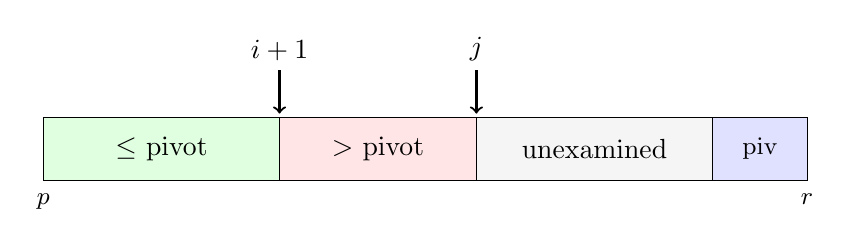
\begin{tikzpicture}[scale=1]
  % four zones
  \draw[fill=green!12] (0,0) rectangle (3,0.8);
  \draw[fill=red!10]   (3,0) rectangle (5.5,0.8);
  \draw[fill=gray!8]   (5.5,0) rectangle (8.5,0.8);
  \draw[fill=blue!12]  (8.5,0) rectangle (9.7,0.8);
  \node at (1.5,0.4) {$\le$ pivot};
  \node at (4.25,0.4) {$>$ pivot};
  \node at (7.0,0.4) {unexamined};
  \node at (9.1,0.4) {\small piv};
  % markers
  \draw[->,thick] (3,1.4) -- (3,0.85);
  \node[above] at (3,1.4) {$i+1$};
  \draw[->,thick] (5.5,1.4) -- (5.5,0.85);
  \node[above] at (5.5,1.4) {$j$};
  \node[below] at (0,-0.05) {\small $p$};
  \node[below] at (9.7,-0.05) {\small $r$};
\end{tikzpicture}
\caption{The Lomuto invariant. Everything before index $i+1$ is $\le$ the pivot;
everything from $i+1$ up to $j-1$ is $>$ the pivot; $A[j \mathinner{\ldotp\ldotp} r-1]$ is not yet
examined; $A[r]$ is the pivot.}
\label{ch07:lomuto-zones}
\end{figure}

Here is the code. Read it once, then we will trace it.

\begin{algorithm}[H]
\caption{\textsc{Partition}($A, p, r$) -- Lomuto scheme}
\KwIn{Subarray $A[p \mathinner{\ldotp\ldotp} r]$ with $p \le r$.}
\KwOut{Returns an index $q$; afterward $A[p \mathinner{\ldotp\ldotp} q-1] \le A[q] < A[q+1 \mathinner{\ldotp\ldotp} r]$.}
$x \leftarrow A[r]$ \tcp*{the pivot is the last element}
$i \leftarrow p - 1$ \tcp*{$i$ = end of the ``$\le$ pivot'' region}
\For{$j \leftarrow p$ \KwTo $r-1$}{
  \If{$A[j] \le x$}{
    $i \leftarrow i + 1$\;
    exchange $A[i]$ with $A[j]$\;
  }
}
exchange $A[i+1]$ with $A[r]$ \tcp*{drop the pivot into place}
\Return $i+1$\;
\end{algorithm}

\subsection{A complete numeric trace}

Let us partition the subarray
\[
A = [\,2,\ 8,\ 7,\ 1,\ 3,\ 5,\ 6,\ 4\,],
\]
with $p = 1$, $r = 8$. The pivot is $x = A[8] = 4$. We start with $i = 0$
(meaning ``the small region is empty''). We will show the array after each
iteration of $j$, marking the pivot in \textbf{bold} and using a vertical bar to
show where $i$ sits (everything up to and including position $i$ is the
$\le$-pivot region).

\begin{labbox}
Trace it with me, but also keep a finger on the page and predict each step
before you read it. The mechanical rule is: \emph{whenever $A[j] \le 4$, bump
$i$ up by one and swap $A[i]$ with $A[j]$; otherwise do nothing and move on.}

\medskip
\begin{tabular}{lll}
\toprule
step & $j$, $A[j]$, decision & array (bar after position $i$) \\
\midrule
start & --- & $\mid 2\ 8\ 7\ 1\ 3\ 5\ 6\ \mathbf{4}$ \\
$j=1$ & $A[1]=2 \le 4$: $i{=}1$, swap $A[1],A[1]$ & $2 \mid 8\ 7\ 1\ 3\ 5\ 6\ \mathbf{4}$ \\
$j=2$ & $A[2]=8 > 4$: skip                        & $2 \mid 8\ 7\ 1\ 3\ 5\ 6\ \mathbf{4}$ \\
$j=3$ & $A[3]=7 > 4$: skip                        & $2 \mid 8\ 7\ 1\ 3\ 5\ 6\ \mathbf{4}$ \\
$j=4$ & $A[4]=1 \le 4$: $i{=}2$, swap $A[2],A[4]$ & $2\ 1 \mid 7\ 8\ 3\ 5\ 6\ \mathbf{4}$ \\
$j=5$ & $A[5]=3 \le 4$: $i{=}3$, swap $A[3],A[5]$ & $2\ 1\ 3 \mid 8\ 7\ 5\ 6\ \mathbf{4}$ \\
$j=6$ & $A[6]=5 > 4$: skip                        & $2\ 1\ 3 \mid 8\ 7\ 5\ 6\ \mathbf{4}$ \\
$j=7$ & $A[7]=6 > 4$: skip                        & $2\ 1\ 3 \mid 8\ 7\ 5\ 6\ \mathbf{4}$ \\
\midrule
final swap & swap $A[i+1]{=}A[4]$ with $A[8]$    & $2\ 1\ 3\ \mathbf{4} \mid 8\ 7\ 5\ 6$ \\
\bottomrule
\end{tabular}

\medskip
The function returns $q = i+1 = 4$. Look at the result:
$[2,1,3]$ are all $\le 4$, the pivot $4$ sits at index $4$, and $[8,7,5,6]$ are
all $> 4$. The pivot is home. Quicksort now recurses on $[2,1,3]$ and $[8,7,5,6]$.
\end{labbox}

Notice the two swaps that actually \emph{moved} things: at $j=4$ the value $1$
(small) traded places with $8$ (large), and at $j=5$ the value $3$ (small)
traded with the $7$ that $8$ had been swapped past. Each time we find a small
element, we swap it into the small region, pushing one large element out into
the large region. The pattern is: \emph{small elements bubble forward, large
elements get shoved back,} and at the very end the pivot jumps over the entire
large region to land right after the small region.

\subsection{Why it is correct: a loop invariant}

We claimed the output satisfies $A[p \mathinner{\ldotp\ldotp} q-1] \le A[q] < A[q+1 \mathinner{\ldotp\ldotp} r]$. The
gentle way to prove it is with a loop invariant: a
statement that is true before the loop starts and stays true after every
iteration. If it survives to the end, it pins down the final
state.

\begin{formalbox}
\textbf{Loop invariant (Lomuto).} At the start of each iteration of the
\textbf{for} loop with loop variable $j$, the following hold:
\begin{enumerate}
\item For every index $k$ with $p \le k \le i$, we have $A[k] \le x$.
\item For every index $k$ with $i+1 \le k \le j-1$, we have $A[k] > x$.
\item $A[r] = x$ (the pivot has not moved).
\end{enumerate}
In words: everything in the small region is $\le$ the pivot, everything in the
large region is $>$ the pivot, and the pivot is still parked at the right end.
\end{formalbox}

\begin{lemma}[Partition correctness]
\label{ch07:lomuto-correct}
After \textsc{Partition}($A,p,r$) returns $q = i+1$, every element of
$A[p \mathinner{\ldotp\ldotp} q-1]$ is $\le A[q]$ and every element of $A[q+1 \mathinner{\ldotp\ldotp} r]$ is $> A[q]$,
where $A[q]$ equals the original pivot value $x$.
\end{lemma}

\begin{proof}
We verify the invariant in three steps.

\emph{Initialization.} Before the first iteration, $j = p$ and $i = p-1$.
Region 1 spans $p \le k \le p-1$, which is empty, so condition 1 holds vacuously.
Region 2 spans $p \le k \le p-1$, also empty, so condition 2 holds vacuously.
And $A[r] = x$ because we have not touched it. The invariant holds.

\emph{Maintenance.} Suppose the invariant holds at the start of an iteration with
loop variable $j$. We look at $A[j]$.
\begin{itemize}
\item If $A[j] > x$: we do nothing but advance $j$. The element at the old
position $j$ now falls into region 2 (indices $i+1$ through the new $j-1$), and
it satisfies $A[j] > x$, so condition 2 still holds. Conditions 1 and 3 are
untouched.
\item If $A[j] \le x$: we increment $i$ and swap $A[i]$ with $A[j]$. The slot
$A[i]$ used to be the first element of region 2, so it held a value $> x$; now it
receives the value $A[j] \le x$, extending region 1 correctly. The displaced
large value lands at the old position $j$, which becomes the new tail of region
2 as $j$ advances, so condition 2 still holds. Condition 3 is untouched because
$j \le r-1 < r$, so we never swap the pivot.
\end{itemize}
In both cases the invariant survives.

\emph{Termination.} The loop ends when $j = r$. By condition 1, all of
$A[p \mathinner{\ldotp\ldotp} i]$ is $\le x$; by condition 2, all of $A[i+1 \mathinner{\ldotp\ldotp} r-1]$ is $> x$.
The final swap exchanges $A[i+1]$ with $A[r] = x$. (When the large region is
nonempty, $A[i+1]$ held a value $> x$; when it is empty, $i+1 = r$ and the swap
is harmless.) After it, $A[i+1] = x$, the values in
$A[p \mathinner{\ldotp\ldotp} i]$ are $\le x$, and the values in $A[i+2 \mathinner{\ldotp\ldotp} r]$ are $> x$ (the
displaced large value joined them). Returning $q = i+1$ makes the claim exact.
\end{proof}

\begin{trapbox}
A subtle point that trips people up: the inequality on the left is $\le$, not
$<$. Elements \emph{equal} to the pivot go to the \emph{left}. That is fine for
correctness, but it matters a great deal for performance. If your array is all
duplicates -- say $n$ copies of the number $5$ -- Lomuto sends \emph{every}
element into the left region, so the partition is maximally unbalanced ($n-1$ on
the left, $0$ on the right) every single time. That is the worst case in
disguise. We will fix this danger later with randomization, and we will see that
Hoare's scheme handles equal keys more gracefully.
\end{trapbox}

\section{The two recursion patterns: best and worst case}

Now that partition is trustworthy, the running time of quicksort is decided
entirely by \emph{how balanced the splits are}. Partitioning a subarray of size
$n$ costs $\Theta(n)$ -- one scan, a constant amount of work per element. The
question is what sizes the two recursive calls get.

\subsection{The worst case: maximally lopsided splits}

Suppose every single partition is as unbalanced as possible: the pivot is always
the smallest (or largest) element, so one side gets $n-1$ elements and the other
gets $0$. When does this happen? Precisely when the array is already sorted (or
reverse sorted) and we keep picking the last element as the pivot. Then the
recurrence for the running time $T(n)$ is
\[
T(n) = T(n-1) + T(0) + \Theta(n) = T(n-1) + \Theta(n).
\]
This unrolls into a sum (the chain in Figure~\ref{ch07:worst-chain}):
\[
T(n) = \Theta(n) + \Theta(n-1) + \cdots + \Theta(2) + \Theta(1)
     = \Theta\!\left(\sum_{k=1}^{n} k\right) = \Theta\!\left(\frac{n(n+1)}{2}\right) = \Theta(n^2).
\]

\begin{figure}[h]
\centering
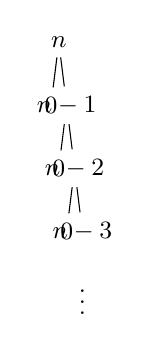
\begin{tikzpicture}[level distance=8mm, sibling distance=2mm,
  every node/.style={font=\small}]
  \node {$n$}
    child {node {$0$}}
    child {node {$n-1$}
      child {node {$0$}}
      child {node {$n-2$}
        child {node {$0$}}
        child {node {$n-3$}
          child[densely dotted] {node {$\vdots$} edge from parent[draw=none]}
        }
      }
    };
\end{tikzpicture}
\caption{The worst-case recursion ``tree'' for quicksort is really a chain of
depth $n$. Each level removes one element and does linear work on the rest, so
the total work is $n + (n-1) + \cdots + 1 = \Theta(n^2)$.}
\label{ch07:worst-chain}
\end{figure}

So the worst case is genuinely $\Theta(n^2)$. This is no better than insertion
sort. If that were the whole story, nobody would use quicksort.

\subsection{The best case: perfectly even splits}

Now suppose we get the opposite luck: every partition splits the subarray into
two halves of size $n/2$ (give or take one for the pivot). Then
\[
T(n) = 2\,T(n/2) + \Theta(n).
\]
This is the merge-sort recurrence, and by the master theorem (Chapter~4) its
solution is $T(n) = \Theta(n \log n)$. The recursion tree has depth $\log_2 n$,
each level does $\Theta(n)$ total work, and $\log_2 n$ levels times $\Theta(n)$
gives $\Theta(n \log n)$. Figure~\ref{ch07:best-tree} shows why the work per
level stays flat at $\Theta(n)$ even as the tree fans out.

\begin{figure}[h]
\centering
\begin{tikzpicture}[level distance=10mm,
  level 1/.style={sibling distance=42mm},
  level 2/.style={sibling distance=21mm},
  every node/.style={font=\small, draw=sourceblue, fill=sourceblue!8,
    rounded corners, inner sep=2pt}]
  \node {$n$}
    child {node {$n/2$}
      child {node {$n/4$}
        child[densely dotted] {node[draw=none,fill=none] {$\vdots$} edge from parent[draw=none]} }
      child {node {$n/4$}
        child[densely dotted] {node[draw=none,fill=none] {$\vdots$} edge from parent[draw=none]} } }
    child {node {$n/2$}
      child {node {$n/4$}
        child[densely dotted] {node[draw=none,fill=none] {$\vdots$} edge from parent[draw=none]} }
      child {node {$n/4$}
        child[densely dotted] {node[draw=none,fill=none] {$\vdots$} edge from parent[draw=none]} } };
  % per-level work annotations
  \node[draw=none,fill=none,anchor=west] at (4.2,0)    {work $=\Theta(n)$};
  \node[draw=none,fill=none,anchor=west] at (4.2,-1)   {$2\cdot\Theta(n/2)=\Theta(n)$};
  \node[draw=none,fill=none,anchor=west] at (4.2,-2)   {$4\cdot\Theta(n/4)=\Theta(n)$};
\end{tikzpicture}
\caption{The best-case recursion tree. Each level holds subproblems whose sizes
sum to $n$, so each level costs $\Theta(n)$. Balanced halving makes the tree only
$\log_2 n$ levels deep, for a total of $\Theta(n \log n)$. Compare the worst-case
chain in Figure~\ref{ch07:worst-chain}, which is $n$ levels deep.}
\label{ch07:best-tree}
\end{figure}

\begin{intuitionbox}
Why does balance matter so much? Think about \emph{depth}. Every level of
recursion does about $\Theta(n)$ work in total (the partitions at that level
collectively scan roughly all $n$ elements). So the running time is essentially
$\Theta(n)$ times the \emph{number of levels}. Balanced splits halve the problem
each level, giving only $\log_2 n$ levels. Lopsided splits shave off one element
per level, giving $n$ levels. That is the entire difference between
$n \log n$ and $n^2$: how fast the subproblems shrink.
\end{intuitionbox}

\subsection{The reassuring middle: even bad balance is fine}

Here is the fact that makes quicksort believable. You do not need \emph{perfect}
balance to get $\Theta(n \log n)$. You just need the split ratio to be bounded
away from the extreme. Suppose every partition is a lopsided $9$-to-$1$ split --
that sounds awful -- so that
\[
T(n) = T\!\left(\tfrac{9n}{10}\right) + T\!\left(\tfrac{n}{10}\right) + \Theta(n).
\]
Draw the recursion tree (Figure~\ref{ch07:lopsided-tree}). The shallowest leaf is
reached by repeatedly taking the $\frac{1}{10}$ branch, at depth $\log_{10} n$.
The deepest leaf is reached by repeatedly taking the $\frac{9}{10}$ branch, at
depth $\log_{10/9} n$. Every \emph{full} level does at most $\Theta(n)$ work, and
there are at most $\log_{10/9} n = \Theta(\log n)$ levels before everything
bottoms out. So the total is at most $\Theta(n \log n)$. A $99$-to-$1$ split
would still give $\Theta(n \log n)$; only the constant inside the $\log$ changes.

\begin{figure}[h]
\centering
\begin{tikzpicture}[level distance=9mm,
  every node/.style={font=\small, draw=quotientorange, fill=quotientorange!10,
    rounded corners, inner sep=2pt},
  edge from parent/.style={draw, -{Latex}}]
  \node {$n$}
    child {node {$\tfrac{1}{10}n$}
      child[densely dotted] {node[draw=none,fill=none] {$\vdots$} edge from parent[draw=none]} }
    child {node {$\tfrac{9}{10}n$}
      child {node {$\tfrac{1}{100}n$}
        child[densely dotted] {node[draw=none,fill=none] {$\vdots$} edge from parent[draw=none]} }
      child {node {$\tfrac{81}{100}n$}
        child[densely dotted] {node[draw=none,fill=none] {$\vdots$} edge from parent[draw=none]} } };
  \node[draw=none,fill=none,anchor=west,font=\footnotesize\itshape]
    at (2.6,-0.9) {shortest path: $\log_{10}n$ levels};
  \node[draw=none,fill=none,anchor=west,font=\footnotesize\itshape]
    at (2.6,-1.9) {longest path: $\log_{10/9}n$ levels};
\end{tikzpicture}
\caption{A consistently $9$-to-$1$ recursion tree. The lightly loaded
$\frac{1}{10}$ branches bottom out quickly ($\log_{10} n$ deep); the heavy
$\frac{9}{10}$ branches form the longest root-to-leaf path ($\log_{10/9} n$
deep). Both depths are $\Theta(\log n)$, and each level still costs $\Theta(n)$,
so the total stays $\Theta(n\log n)$.}
\label{ch07:lopsided-tree}
\end{figure}

\begin{focusbox}
The lesson: quicksort is $\Theta(n \log n)$ unless the splits are
\emph{consistently, catastrophically} lopsided -- close to $0$-to-$n$ almost
every time. A merely ``unlucky'' split here and there costs you nothing
asymptotically. This robustness is the seed of why randomization rescues
quicksort: random pivots make consistent catastrophe astronomically unlikely.
\end{focusbox}

\section{The villain in the input, and how to remove it}

So far we have chosen the pivot as $A[r]$, the last element. That choice has a
fatal flaw: it makes the running time depend on the \emph{arrangement of the
input}. An already-sorted array -- one of the most common inputs in the real
world -- triggers the $\Theta(n^2)$ worst case every time. That is a disaster.
Imagine a database that re-sorts an already-sorted log file and grinds to a halt.

\begin{trapbox}
The naive fix people reach for first is ``pick the middle element'' or ``pick
the first element.'' These help against sorted inputs but do not solve the
problem: for \emph{any} fixed deterministic rule for choosing the pivot, an
adversary who knows your rule can construct an input that forces the worst case.
There is always a bad input. The only escape is to stop letting the input
decide.
\end{trapbox}

The cure is a classic move in algorithm design: make the pivot
\emph{random}. Instead of always taking $A[r]$, pick a uniformly random index
between $p$ and $r$, swap that element into position $r$, and proceed exactly as
before. The partition logic is unchanged; only the pivot's identity is now a
coin flip.

\begin{algorithm}[H]
\caption{\textsc{Randomized-Partition}($A, p, r$)}
\KwIn{Subarray $A[p \mathinner{\ldotp\ldotp} r]$.}
\KwOut{A partition around a uniformly random pivot; returns the pivot index.}
$s \leftarrow \textsc{Random}(p, r)$ \tcp*{uniform in $\{p, \dots, r\}$}
exchange $A[r]$ with $A[s]$ \tcp*{move random pivot to the end}
\Return $\textsc{Partition}(A, p, r)$\;
\end{algorithm}

\begin{algorithm}[H]
\caption{\textsc{Randomized-Quicksort}($A, p, r$)}
\If{$p < r$}{
  $q \leftarrow \textsc{Randomized-Partition}(A, p, r)$\;
  $\textsc{Randomized-Quicksort}(A, p, q-1)$\;
  $\textsc{Randomized-Quicksort}(A, q+1, r)$\;
}
\end{algorithm}

\begin{aestheticbox}
This shifts what ``worst case'' even means. With deterministic
quicksort, the worst case is a property of the \emph{input}: a specific evil
array. With randomized quicksort, \emph{no input is reliably bad}. For any fixed
array, the running time becomes a random variable, and we will prove
its \emph{expected} value is $\Theta(n \log n)$ regardless of how the input was
arranged. The randomness lives in the algorithm's coin flips, not in the data.
An adversary can choose the array but cannot see your coins. The same trick --
randomize to defeat worst-case inputs -- shows up all over computer science: in
hashing (Chapter~11), in load balancing, in cryptography.
\end{aestheticbox}

\begin{historybox}
Quicksort was invented by Tony Hoare in 1959--1961 while he was a young
researcher trying to sort words for a machine-translation project in Moscow. He
later won the Turing Award. The randomized-pivot and rigorous expected-time
analysis are developed carefully in \textbf{CLRS Chapter 7} (``Quicksort''),
with the indicator-variable argument in \textbf{Section 7.4.2}. The Lomuto
partition we used is in \textbf{Section 7.1}; Hoare's original partition is
explored in \textbf{Problem 7-1}. Read this chapter first and CLRS 7 will read
like review.
\end{historybox}

\section{The heart of the matter: expected running time}

We now prove the central theorem. This is the analysis the chapter has been
building toward, and once it clicks it tends to stay with you.

\begin{theorem}[Expected time of randomized quicksort]
\label{ch07:expected-time}
On any input of $n$ distinct elements, \textsc{Randomized-Quicksort} runs in
expected time $O(n \log n)$, where the expectation is over the random choices of
pivots.
\end{theorem}

The whole running time of quicksort is dominated by one operation:
\emph{comparing an element to a pivot} inside \textsc{Partition}. Every other
operation (swaps, index bookkeeping, recursive call overhead) is bounded by a
constant times the number of partition calls, and there are at most $n$ partition
calls total. So bounding the \emph{total number of comparisons} $X$ across
the entire run bounds the running time, which is $O(n + X)$.

\begin{focusbox}
The entire analysis reduces to one question: \emph{across the whole sort, how
many times does the algorithm compare two elements?} Count the comparisons and
you have the running time. We will count them with a clever trick called
\emph{indicator random variables}.
\end{focusbox}

\subsection{The key realization: each pair is compared at most once}

Rename the elements by their \emph{sorted order}, not their positions in
the input. Let $z_1 < z_2 < \cdots < z_n$ be the elements in sorted order, so
$z_i$ is the $i$-th smallest. Define $Z_{ij} = \{z_i, z_{i+1}, \dots, z_j\}$, the
set of elements whose sorted ranks fall between $i$ and $j$ inclusive.

\begin{intuitionbox}
Here is the linchpin observation. When are two elements $z_i$ and $z_j$ ever
\emph{directly compared}? Comparisons only happen between a pivot and a
non-pivot. So $z_i$ and $z_j$ are compared if and only if one of them is chosen
as a pivot \emph{while they are still in the same subarray}. And crucially, once
two elements are compared, one of them was the pivot, which then leaves the
recursion -- so \textbf{any pair is compared at most once} in the entire run.
\end{intuitionbox}

Now ask \emph{which} element, chosen as a pivot, would either compare
$z_i$ with $z_j$ or else separate them forever. Consider the set $Z_{ij}$. As
long as no element of $Z_{ij}$ has been chosen as a pivot, all of $Z_{ij}$ sits
together in one subarray (because any pivot \emph{outside} $Z_{ij}$ is either
smaller than every $z$ in $Z_{ij}$, sending them all right, or larger than every
one, sending them all left -- never splitting them). The first pivot chosen
\emph{from within} $Z_{ij}$ decides their fate:
\begin{itemize}
\item If that first pivot is $z_i$ or $z_j$ itself, then $z_i$ and $z_j$
\emph{are} compared (the pivot is compared against every other element in the
subarray, including the other one).
\item If that first pivot is some \emph{middle} element $z_k$ with $i < k < j$,
then $z_i$ goes to the left subarray and $z_j$ goes to the right subarray. They
are now separated forever and will \emph{never} be compared.
\end{itemize}

So $z_i$ and $z_j$ are compared if and only if the \emph{first} element chosen as
a pivot from the set $Z_{ij}$ is either $z_i$ or $z_j$.
Figure~\ref{ch07:zij} lays out the three cases on a number line of sorted ranks.

\begin{figure}[h]
\centering
\begin{tikzpicture}[font=\small]
  % the sorted rank axis
  \draw[-{Latex}] (-0.5,0) -- (10,0) node[right] {sorted rank};
  % Z_ij block
  \draw[fill=structurepurple!12, draw=structurepurple]
        (3,-0.25) rectangle (7,0.25);
  \node[structurepurple, above] at (5,0.3) {$Z_{ij}$};
  % endpoints and a middle
  \foreach \x/\lab in {1/{}, 3/{z_i}, 5/{z_k}, 7/{z_j}, 9/{}} {
    \fill (\x,0) circle (1.6pt);
  }
  \node[below] at (3,-0.3) {$z_i$};
  \node[below] at (5,-0.3) {$z_k$};
  \node[below] at (7,-0.3) {$z_j$};
  \node[below] at (1,-0.3) {$<z_i$};
  \node[below] at (9,-0.3) {$>z_j$};
  % verdicts
  \node[targetgreen, anchor=west] at (-0.5,1.15)
    {\textbf{First pivot $=z_i$ or $z_j$:} the two are compared.};
  \node[trapred, anchor=west] at (-0.5,0.75)
    {\textbf{First pivot $=z_k$ (middle):} $z_i$ and $z_j$ split apart, never compared.};
\end{tikzpicture}
\caption{The fate of the pair $(z_i, z_j)$ is sealed by the first pivot drawn
from the contiguous rank-block $Z_{ij}$. A pivot from \emph{outside} the block
(rank $<z_i$ or $>z_j$) pushes the whole block to one side without splitting it,
so it never decides anything. An endpoint pivot compares the pair; a strictly
interior pivot $z_k$ separates them forever.}
\label{ch07:zij}
\end{figure}

\begin{walkbox}
Before reading the probability calculation, take this on a walk. The set
$Z_{ij}$ has exactly $j - i + 1$ elements. Each pivot is chosen uniformly at
random, so before any of $Z_{ij}$ has been a pivot, each of its $j-i+1$ members
is \emph{equally likely} to be the first one chosen from the set. We want the
chance that the first one is one of the \emph{two} endpoints, $z_i$ or $z_j$.
Two favorable outcomes out of $j-i+1$ equally likely ones. Can you guess the
probability before we derive it?
\end{walkbox}

\subsection{Indicator variables and the count}

Define the indicator random variable
\[
X_{ij} = \mathbb{I}\{z_i \text{ is compared with } z_j \text{ at some point during the sort}\}
       = \begin{cases} 1 & \text{if they are compared}, \\ 0 & \text{otherwise}. \end{cases}
\]
Since every pair is compared at most once, the total number of comparisons is
exactly
\[
X = \sum_{i=1}^{n-1} \sum_{j=i+1}^{n} X_{ij}.
\]
We want $\E[X]$, the expected number of comparisons. By \emph{linearity of
expectation} -- which holds whether or not the variables are independent, a fact
worth treasuring --
\[
\E[X] = \E\!\left[\sum_{i=1}^{n-1}\sum_{j=i+1}^{n} X_{ij}\right]
      = \sum_{i=1}^{n-1}\sum_{j=i+1}^{n} \E[X_{ij}]
      = \sum_{i=1}^{n-1}\sum_{j=i+1}^{n} \Pr[z_i \text{ compared with } z_j].
\]
The last equality is the defining property of an indicator: its expectation
equals the probability of the event it indicates.

Now we compute that probability using the realization above. Among the $j-i+1$
elements of $Z_{ij}$, each is equally likely to be the first chosen as a pivot.
The comparison happens exactly when that first pivot is $z_i$ or $z_j$:
\[
\Pr[z_i \text{ compared with } z_j]
   = \frac{2}{j - i + 1}.
\]

\begin{formalbox}
\textbf{Why the probability is $\dfrac{2}{j-i+1}$.} Restrict attention to the
moment when the first pivot \emph{from $Z_{ij}$} is selected. By symmetry of the
uniform random pivot choice, each of the $j-i+1$ elements of $Z_{ij}$ is equally
likely to be that first one, each with probability $\frac{1}{j-i+1}$. The event
``compared'' is the union of the two disjoint events ``$z_i$ is first'' and
``$z_j$ is first,'' so its probability is $\frac{1}{j-i+1} + \frac{1}{j-i+1} =
\frac{2}{j-i+1}$.
\end{formalbox}

\subsection{Summing the series}

Substitute, and let $k = j - i$ so that as $j$ ranges from $i+1$ to $n$, $k$
ranges from $1$ to $n - i$:
\[
\E[X] = \sum_{i=1}^{n-1}\sum_{j=i+1}^{n} \frac{2}{j-i+1}
      = \sum_{i=1}^{n-1}\sum_{k=1}^{n-i} \frac{2}{k+1}
      < \sum_{i=1}^{n-1}\sum_{k=1}^{n} \frac{2}{k}.
\]
The inner sum $\sum_{k=1}^{n} \frac{1}{k}$ is the $n$-th \emph{harmonic number}
$H_n$, and a fact we will lean on (proved in the summations appendix, and in
CLRS) is that $H_n = \ln n + O(1) = O(\log n)$. Therefore
\[
\E[X] < \sum_{i=1}^{n-1} 2 H_n = \sum_{i=1}^{n-1} O(\log n) = O(n \log n).
\]
Since the running time is $O(n + X)$ and $\E[X] = O(n \log n)$, the expected
running time is $O(n \log n)$. This proves Theorem~\ref{ch07:expected-time}.
\hfill$\square$

\begin{intuitionbox}
Look at what just happened. We did not solve a recurrence. We did
not draw a recursion tree. We \emph{counted comparisons one pair at a time}, and
the only thing we needed about each pair was the chance that the two ever
meet. Distant pairs (large $j - i$) almost never meet -- the probability
$\frac{2}{j-i+1}$ shrinks toward zero -- while adjacent pairs (small $j-i$) meet
often. Summing those probabilities gives the harmonic series, which is
$\Theta(\log n)$. That logarithm is the whole reason quicksort is fast,
and it was hiding in the harmonic numbers all along.
\end{intuitionbox}

\begin{remark}
Why the harmonic number? Because the probability $\frac{2}{j-i+1}$ depends only
on the \emph{gap} $j - i$ between the ranks. For each fixed gap $d$, there are
about $n$ pairs at that gap, each contributing $\frac{2}{d+1}$, giving roughly
$\frac{2n}{d+1}$. Summing over gaps $d = 1, 2, \dots, n-1$ produces $2n$ times
the harmonic series -- exactly the $\Theta(n \log n)$ we found. The structure of
the answer is built into the geometry of ranks.
\end{remark}

\section{Hoare partitioning: the original, faster scheme}

Lomuto is easy to reason about, but Hoare's original 1961 partition is
typically \emph{faster in practice} because it does fewer swaps -- on average
about three times fewer. It works by sending two fingers toward each other from
the two ends, swapping out-of-place pairs as they meet.

\begin{algorithm}[H]
\caption{\textsc{Hoare-Partition}($A, p, r$)}
\KwIn{Subarray $A[p \mathinner{\ldotp\ldotp} r]$ with $p < r$.}
\KwOut{An index $q \in \{p, \dots, r-1\}$ splitting $A$ so that $A[p \mathinner{\ldotp\ldotp} q]$ all $\le$ $A[q+1 \mathinner{\ldotp\ldotp} r]$.}
$x \leftarrow A[p]$ \tcp*{pivot = first element}
$i \leftarrow p - 1$\;
$j \leftarrow r + 1$\;
\While{\textbf{true}}{
  \Repeat{$A[j] \le x$}{$j \leftarrow j - 1$}
  \Repeat{$A[i] \ge x$}{$i \leftarrow i + 1$}
  \eIf{$i < j$}{
    exchange $A[i]$ with $A[j]$\;
  }{
    \Return $j$\;
  }
}
\end{algorithm}

\begin{intuitionbox}
The two fingers $i$ and $j$ march toward each other. The left finger $i$ stops
when it finds an element that is too big (it belongs on the right). The right
finger $j$ stops when it finds an element too small (it belongs on the left).
Then they swap, fixing two misplaced elements at once. They keep going until the
fingers cross. Where they cross is the boundary: everything at or left of $j$ is
$\le$ the pivot, everything right of $j$ is $\ge$ it.
\end{intuitionbox}

\begin{trapbox}
Hoare partition has two gotchas that Lomuto does not. First, the returned index
$q$ is \emph{not} the pivot's final resting place -- the pivot may still be
loose somewhere in the left part. So the recursive calls differ: you call
$\textsc{Quicksort}(A, p, q)$ and $\textsc{Quicksort}(A, q+1, r)$ -- note $q$ is
\emph{included} in the left call, and there is no ``$q-1$'' or ``$q+1$''
skipping a pivot. Second, you must choose the pivot as $A[p]$ (the first
element), not $A[r]$; choosing $A[r]$ can cause the loop to run off the end of
the array. These off-by-one and boundary subtleties are exactly why textbooks
teach Lomuto first.
\end{trapbox}

\begin{labbox}
Trace \textsc{Hoare-Partition} on $A = [\,5,\ 3,\ 8,\ 1,\ 9,\ 2,\ 7\,]$,
$p=1$, $r=7$, pivot $x = A[1] = 5$.

\medskip
{\small\setlength{\tabcolsep}{4pt}
\begin{tabular}{lll}
\toprule
fingers stop at & comparison & action \\
\midrule
$j$: $7,2$ stop at $A[6]{=}2 \le 5$; $i$: stop at $A[1]{=}5 \ge 5$ & $i{=}1 < j{=}6$ & swap $A[1],A[6]$: $[2,3,8,1,9,5,7]$ \\
$j$: $9,1$ stop at $A[4]{=}1$; $i$: $3,8$ stop at $A[3]{=}8$ & $i{=}3 < j{=}4$ & swap $A[3],A[4]$: $[2,3,1,8,9,5,7]$ \\
$j$: stop at $A[3]{=}1$; $i$: stop at $A[4]{=}8$ & $i{=}4 \not< j{=}3$ & return $q = 3$ \\
\bottomrule
\end{tabular}}

\medskip
Final array $[2,3,1,\,8,9,5,7]$ with $q=3$. Check: $A[1\mathinner{\ldotp\ldotp} 3]=[2,3,1]$ are all
$\le 5$, and $A[4 \mathinner{\ldotp\ldotp} 7]=[8,9,5,7]$ are all $\ge 5$. The split is valid even
though the pivot $5$ is sitting at index $6$, not at the boundary. That is why
the recursion includes index $q$ on the left.
\end{labbox}

\begin{aestheticbox}
Why does industry care which partition scheme is used if both are
$\Theta(n \log n)$ on average? Because the constant factor shows up on the clock.
A swap moves data in memory; fewer swaps mean fewer cache misses and fewer writes.
Hoare's scheme does about $\frac{1}{3}$ as many swaps as Lomuto's, which is why
high-performance library sorts (and hybrids like \emph{introsort}, used in C++'s
\lstinline|std::sort|) build on Hoare-style partitioning. The asymptotics tell
you the shape of the curve; the constants tell you who wins the benchmark.
\end{aestheticbox}

\section{Engineering the real thing}

A production quicksort is rarely the textbook version verbatim. A handful of
refinements turn the idea into a top-tier sort:

\begin{itemize}
\item \textbf{Cut over to insertion sort for tiny subarrays.} When a subarray
drops below, say, $10$--$16$ elements, insertion sort (Chapter~2) beats
quicksort because its constant factors are tiny and it has no recursion
overhead. Many implementations stop recursing at small sizes and finish with a
single insertion-sort pass over the whole nearly-sorted array.
\item \textbf{Median-of-three pivoting.} Instead of a random or fixed pivot,
take the median of $A[p]$, $A[r]$, and the middle element. This makes a balanced
split far more likely on real-world data and is cheap.
\item \textbf{Three-way partitioning for duplicates.} Recall the trap: arrays
with many equal keys destroy basic quicksort. A \emph{three-way} partition
(``Dutch national flag'') splits into $< x$, $= x$, and $> x$ regions, so all
copies of the pivot are placed at once and never recursed on. This turns the
all-duplicates worst case into linear time.
\item \textbf{Bounded recursion depth (introsort).} To guarantee
$O(n \log n)$ even in the worst case, monitor the recursion depth; if it exceeds
$\approx 2\log_2 n$, bail out to heapsort (Chapter~6) for that subarray. You keep
quicksort's speed on typical inputs and heapsort's worst-case guarantee. This
hybrid is \emph{introsort}, the basis of the C++ standard library sort.
\end{itemize}

\begin{complexitybox}
\textbf{Quicksort at a glance} (sorting $n$ elements).
\begin{center}
\begin{tabular}{lll}
\toprule
Quantity & Value & When \\
\midrule
Best-case time            & $\Theta(n \log n)$ & balanced splits \\
Average / expected time   & $\Theta(n \log n)$ & random pivots, distinct keys \\
Worst-case time           & $\Theta(n^2)$      & always-lopsided splits \\
Auxiliary space           & $\Theta(\log n)$ expected & recursion stack \\
In place?                 & yes (no scratch array) & --- \\
Stable?                   & no (swaps reorder equal keys) & --- \\
Comparisons (expected)    & $\approx 2 n \ln n \approx 1.39\, n \log_2 n$ & from $2 H_n$ analysis \\
\bottomrule
\end{tabular}
\end{center}
The expected comparison count $2 n \ln n \approx 1.39\, n \log_2 n$ is only about
$39\%$ above the information-theoretic floor of $\log_2(n!) \approx n \log_2 n$
comparisons that \emph{any} comparison sort must pay (Chapter~8). Quicksort is
nearly optimal in comparisons \emph{and} pays a small constant, which is the
practical magic.
\end{complexitybox}

\begin{trapbox}
``In place'' but watch the stack. Quicksort uses no auxiliary \emph{array}, but
it does use the call stack for recursion, $\Theta(\log n)$ deep when balanced and
$\Theta(n)$ deep in the worst case -- enough to overflow the stack on a large
adversarial input. The fix is \emph{tail-recursion elimination}: always recurse
on the \emph{smaller} side first and loop on the larger side, which caps the
stack at $\Theta(\log n)$ even in the worst case. Library implementations do
this.
\end{trapbox}

\section{Putting it all together}

\begin{focusbox}
The five things to carry out of this chapter:
\begin{enumerate}
\item \textbf{Partition is the engine.} It places one pivot in its final spot in
$\Theta(n)$ time; the combine step is free. That is what makes quicksort sort in
place.
\item \textbf{Balance is everything.} Running time is $\Theta(n)$ times the
recursion depth. Balanced splits give depth $\log n$; lopsided splits give depth
$n$. Even $99$-to-$1$ splits stay $\Theta(n\log n)$.
\item \textbf{Determinism is the enemy.} Any fixed pivot rule has a bad input.
Already-sorted data breaks ``last-element'' pivoting.
\item \textbf{Randomization removes the villain.} Random pivots make the
expected time $\Theta(n \log n)$ on \emph{every} input. The randomness is in your
coins, not the data.
\item \textbf{The proof counts comparisons.} Each pair $z_i, z_j$ is compared
with probability $\frac{2}{j-i+1}$; summing gives harmonic numbers, hence
$\Theta(n \log n)$.
\end{enumerate}
\end{focusbox}

You now understand quicksort more deeply than most people who use it daily. When
you open CLRS Chapter 7, you will recognize every move -- the loop invariant, the
recursion-tree intuition, and especially that indicator-variable
argument.

\section{Exercises}

\begin{exercise}[Trace Lomuto]
Run \textsc{Partition} (Lomuto) by hand on
\[
A = [\,13,\ 19,\ 9,\ 5,\ 12,\ 8,\ 7,\ 4,\ 11,\ 2,\ 6,\ 21\,]
\]
with pivot $A[12] = 21$, then again on the same array
with pivot $A[12]$ replaced by $6$ (swap the $6$ into the last slot first). Show
the array after every iteration of $j$ and give the returned index $q$.
\end{exercise}

\begin{exercise}[Counting in the worst case]
Exactly how many comparisons does Lomuto \textsc{Partition} make on a single call
to a subarray of size $n$? Using this, write and solve the recurrence for the
total number of comparisons quicksort makes when every split is maximally
unbalanced, and confirm it is $\Theta(n^2)$.
\end{exercise}

\begin{exercise}[Best case is no accident]
Suppose \textsc{Partition} always returned an index $q$ exactly in the middle of
the subarray. Write the recurrence and use the master theorem (Chapter~4) to
solve it. Then suppose instead that $q$ always lands at the $\frac{1}{4}$ point
(a $1$-to-$3$ split). Draw the recursion tree, bound its depth, and argue the
total is still $\Theta(n \log n)$.
\end{exercise}

\begin{exercise}[The duplicate-key disaster]
Let $A$ be an array of $n$ identical elements. Trace what Lomuto
\textsc{Partition} does, and determine the exact split sizes it produces. Conclude
that basic quicksort runs in $\Theta(n^2)$ on all-equal input even with a random
pivot. Then describe, in words, how three-way (Dutch-flag) partitioning fixes
this.
\end{exercise}

\begin{exercise}[Hoare hands-on]
Trace \textsc{Hoare-Partition} on $A = [\,4,\ 7,\ 2,\ 9,\ 1,\ 6,\ 3\,]$ with
pivot $A[1]=4$. Show the fingers $i$, $j$ and the array after each swap, and give
the returned $q$. Verify that everything in $A[1 \mathinner{\ldotp\ldotp} q]$ is $\le$ everything in
$A[q+1 \mathinner{\ldotp\ldotp} r]$. Where did the pivot end up?
\end{exercise}

\begin{exercise}[Why the indicator trick works]
In the expected-time proof we claimed that two elements $z_i$ and $z_j$ are
compared if and only if the first pivot chosen from $Z_{ij} = \{z_i, \dots,
z_j\}$ is one of the two endpoints. Explain carefully why a pivot chosen from
\emph{outside} $Z_{ij}$ never separates $z_i$ from $z_j$, and why a middle
element $z_k$ ($i < k < j$) chosen first guarantees they are never compared.
\end{exercise}

\begin{exercise}[Probability of comparing extremes]
Using the formula $\Pr[z_i \text{ compared with } z_j] = \frac{2}{j-i+1}$,
compute the probability that the smallest and the largest elements ($z_1$ and
$z_n$) are ever directly compared, as a function of $n$. What is this probability
for $n = 10$, $n = 100$, $n = 1000$? What does the trend tell you intuitively?
\end{exercise}

\begin{exercise}[Expected comparisons, exactly]
Show that the expected number of comparisons can be written exactly as
$\E[X] = \sum_{i=1}^{n-1}\sum_{k=1}^{n-i} \frac{2}{k+1}$. For $n = 4$, evaluate
this sum by hand to a fraction. (You should get $\frac{2}{2}+\frac{2}{3}+
\frac{2}{4}+\frac{2}{2}+\frac{2}{3}+\frac{2}{2}$ once you list all pairs --
organize them and add.)
\end{exercise}

\begin{exercise}[Tail recursion and stack depth]
Explain why recursing on the \emph{smaller} subarray first and looping on the
larger one bounds the recursion-stack depth to $\Theta(\log n)$ even in the
$\Theta(n^2)$-time worst case. Hint: each time you push a stack frame, the
remaining problem is at most half the size. (Challenge.)
\end{exercise}

\begin{exercise}[Randomized vs.\ shuffle-then-sort]
Some people achieve the benefits of a random pivot by first randomly
\emph{permuting} the entire input array and then running plain (deterministic,
last-element-pivot) quicksort. Argue that this gives the same expected running
time $\Theta(n \log n)$. What is one practical advantage of choosing random
pivots \emph{during} the recursion instead of shuffling up front? (Challenge.)
\end{exercise}

\begin{exercise}[Median-of-three by hand]
For the array $A = [\,8,\ 1,\ 4,\ 9,\ 6,\ 3,\ 5,\ 2,\ 7\,]$, compute the
median-of-three pivot using $A[1]$, the middle element $A[5]$, and $A[9]$. Then
argue, in a sentence or two, why median-of-three makes the already-sorted worst
case essentially impossible to trigger by accident. (Warmup-to-medium.)
\end{exercise}
